

\documentclass{article}
\usepackage{fontspec}
\usepackage{zhspacing,url,amsmath,amssymb,verbatim}
\zhspacing
\usepackage{listings}
\usepackage[hyperfootnotes=false,colorlinks,linkcolor=blue,anchorcolor=blue,citecolor=blue]{hyperref}
\usepackage[sorting=none]{biblatex}
\usepackage{minted}
\usepackage{subfigure}
\usepackage{indentfirst}
\usepackage{cases}
\usepackage{environ}
\usepackage{array}
\usepackage{graphicx}
\usepackage[top=1in, bottom=1in, left=1.25in, right=1.25in]{geometry}

\newcommand{\inputmintedConfigured}[3][]{\inputminted[fontsize=\footnotesize,
	label=#3,linenos,frame=lines,framesep=0.8em,tabsize=4,#1]{#2}{#3}}

\newcommand{\txtsrc}[2][]{\inputmintedConfigured[#1]{text}{#2}}
\newcommand{\txtsrcpart}[4][]{\txtsrc[firstline=#3,firstnumber=#3,lastline=#4,#1]{#2}}

\newcommand{\cppsrc}[2][]{\inputmintedConfigured[#1]{cpp}{#2}}
\newcommand{\cppsrcpart}[4][]{\cppsrc[firstline=#3,firstnumber=#3,lastline=#4,#1]{#2}}


\newcommand{\figref}[1]{\hyperref[fig:#1]{Figure\ref*{fig:#1}}}
\newcommand{\tableref}[1]{\hyperref[table:#1]{Table\ref*{table:#1}}}
\newcommand{\centerize}[1]{\begin{center} #1 \end{center}}

\newcommand{\cmd}[1]{{\it #1}}
\newcommand{\ccmd}[1]{\centerize{\cmd{#1}}}

\title{N-body Simulation using OpenMP, Pthread and MPI}
\author{Xin Huang\\ Dept. of CST, THU\\ ID: 2011011253}
\date{\today}

\addbibresource{refs.bib}
\begin{document}
\maketitle

\newcommand{\nbs}{ {\bf N-body Simulation}  }
\newcommand{\pthread} { {\it pthread} }
\newcommand{\openmp} { {\it OpenMP} }
\newcommand{\mpi} { {\it MPI} }


\begin{abstract}
	An \nbs ~is a simulation of a dynamical system of particles under
	the influence of gravity.\cite{wiki_nbs}
	Here the author compare efficiency among programs using three kinds of
	parallel backends: \openmp, \pthread, and \mpi.

	This is {\it homework 4} for course {\it Parallel Programming}

	{\bf Keyword} N-body, simulation, parallel
\end{abstract}

\tableofcontents

\clearpage

\section{Instruction}
	You can simply follow $make->make~run$ to run the program. For more
	detailed instruction, seed Appedix~\ref{command_line_help}

\section{Design \& Approach}
	\subsection{Definitions}
		\begin{itemize}
			\item {\bf Body}
				The bodies are defined as sphere. A body has its mass, position
				and velocity. All of them are in three dimension. But the demo
				showed in 2 dimension.

			\item {\bf Engine}
				The engine is responsible for the calculation of the gravitational
				effect assigned to the single body and the collision between bodies.

			\item {\bf Worker}
				The worker is responsible for the scheduling the task of calculation
				of the collision and gravity. In this program, there are three
				method to achieve this goal: {\bf OpenMP}, {\bf pthread}, {\bf MPI}.

		\end{itemize}

	\subsection{Overview}
		Simulation consists of multiple rounds. In each round, program
		simulates the state of the system within $\Delta t$ seconds, with the
		approximation of considering the motion as uniform linear motion within
		a round.

		Each round consists of two phases:
		\begin{enumerate}
			\item
				Firstly, we calculate the net force as well as the acceleration
				of one body, and then get the velocity of each. Then we update
				the new position where the body should be.
			\item
				Secondly, we need to consider the collisions between two bodies.
				We know it may be true that more than two bodies can collide
				at the same time. However, too many collision at the same time
				may be trouble for programming for the velocity is unable to
				calculate. So we assume every time of update only one collision
				occurs. The method is to calculate the least time that the bodies
				will collide and calculate that time. And there is a lot of
				calculation to solve the quadric equations. It takes so much
				time.

		\end{enumerate}

	\subsection{The Engine}
		There are two engines available:
			\subsubsection{SimpleEngine}

				SimpleEngine will calculate accelaration {\bf precisely}:
				accumulate all forces exerted on it using formula
				\centerize{$F_{net} = \Sigma \dfrac{G \cdot m \cdot m_{other}}{r^2}$}
				and the accelaration with
				\centerize{$a_{net} = \Sigma \dfrac{F_{net}}{m} = \Sigma \dfrac{G \cdot m_{other}}{r^2} $}
				then the new velocity will be
				\centerize{$v\prime = v + a_{net} * \Delta t$}

				The method use a loop to enumerate all bodie and collisions
				with boundaries. And calculate the least time of the next one
				collision.
				Due to the method enumerate all bodies and in each loop check
				all the other bodies. this method gives an $O(n^2 + n^2) = O(n^2)$
				algorithm for $n$ bodies.

			\subsubsection{BSPTree}

				Comparing to Octree, BSPTree (Binary Space Partitioning Tree)
				is a data structure can arrange bodies in a unlimited space,
				while the former only deals with bounded space. It is easier
				for BSPTree to calculate the position quickly.

				A node in tree holds information of the subtree rooted on that
				node.
				Here are details of the tree:
				\begin{description}
					\item {\bf Axis Aligned Bounding Box(AABox)}

						AABox is a cuboid which can described the bodies set.
						AABox has three perpendicular axis: x, y, z. The objects
						are in this Axis Aligned Bounding Box.

						It's generally used in 3D games.

					\item {\bf Construction of the tree}

						The tree is recursively constructed from the root with
						all bodies given.
						\begin{enumerate}
							\item
								An AABox need to hold the bodies and it's
								attributes, such as the mass and the center
								mass of a box. It can make the calculation
								quicker.
							\item
								Select one axis, and find out the center of
								the bodies in the AABox on this axis.
							\item
								Find out the id of the body in the middle,
								divide the bodies in the AABox into two equal
								parts. The two parts are regarded as the two
								child nodes of the current node. The plane
								divides the box is also in that node.

							\item recursively construct the tree with the two
								parts of the bodies.
						\end{enumerate}

						With $O(n)$ algorithm to find the median, and
						$O(\log{n})$ depth of the tree, construction of the
						tree can be done in $O(n \log{n})$ time. And with
						apparently $O(n)$ nodes in the tree with constant
						information stored on each node, space complexity is
						$O(n)$.

					\item {\bf Acceleration Calculation}

						For each body, we calculate the accelaration its own
						exerted by other bodies start from the root of the
						tree as follow.

						\begin{enumerate}
							\item
								There are a lot of calculation in the accumulation.
								So we need to do some tricks on it.

								We can consider a box of bodies as a mass point
								when the box is so far away from the given body.
								If a node is a leaf node containing one body
								or not a leaf but so far away. We can just
								calculate the mass center to find out the acceleration.

								Here we define the insignificance $\theta$ of a
								node to a body as: \centerize{$\theta =
								\dfrac{V}{D^3}$} where $V$ is the volume of
								AABox of the node, and $D$ is the distance
								between CM of the node and the body.

								We also set a threshold $\eta$ empirically, and
								consider nodes whose $\theta < \eta$ as
								insignificant to the given body.  The large
								$\eta$, the faster and imprecise the
								calculation will be.

							\item
								Else consider the acceleration separately on
								each child node.
						\end{enumerate}

						With certain value of $\eta$, we can expect a much less
						time for each body to obtain its acceleration, expecting
						a $O(n \log{n})$ time complexity.

					\item {\bf Body Collision}

						We can assume the motion in $\delta$t is linear for the
						body collision. And we can quickly detect whether there
						is a collision by distending the AABox a length from
						time 0 to time $\delta$t.

						For each body, we find its earliest collision may
						happen with another body in $\delta t$ time in the tree
						start with root node as follow:
						\begin{enumerate}
							\item construct a new AABox which is the AABox of
								current node but with a expand in width of the
								body's diameter.
							\item if $l_i$ does not intersect the new AABox of
								current node, no further inspection is needed,
								thus return to its root node.
							\item if current node is a leaf node, calculate the
								collision.
							\item if $l_i$ intersect the new AABox of current node,
								inspect both of its child node for further
								investigation.
						\end{enumerate}

						Also, only a few amount of node need to be checked,
						much less time is consumed. If the speed of the body
						is not that large comparing to the volume of AABox,
						this algorithm yields a time complexity of
						$O(n \log{n})$

						We assume two body $b_i$ and $b_j$ will hit at time
						$t$, then we have equations
						$$
							\left \{
								\begin{aligned}
									\mathbf{p_i \prime} &= \mathbf{p_i}
										+ \mathbf{v_i} \cdot t \\
									\mathbf{p_j \prime} &= \mathbf{p_j}
										+ \mathbf{v_j} \cdot t \\
									|\mathbf{p_i} - \mathbf{p_j}| &= r_i + r_j
								\end{aligned}
							\right .
						$$
						where $\mathbf{p_i},\mathbf{v_i},r_i$ are the position,
						velocity and radius of $b_i$ respectively.
						This is a quadric equation set, and we can simply
						choose the smallest opposite $t$ as the solution. If
						such $t$ does not exist or $t > \Delta t$, then the two
						body will not collide.

						Finally, when knowing the two body will collide, the
						response to collision of two body $b_1$ and $b_2$ is
						calculated as follow\cite{col_rspns}:
						$$
							\begin{aligned}
								\mathbf{u} &= \dfrac{\mathbf{p_1} -
								\mathbf{p_2}}{|\mathbf{p_1} - \mathbf{p_2}|} \\
								u_1 &= \mathbf{u} \cdot \mathbf{v_1} \\
								\mathbf{v_{1x}} &= \mathbf{u} \cdot u_1 \\
								\mathbf{v_{1y}} &= \mathbf{v_1} - \mathbf{v_{1x}} \\
								u_2 &= \mathbf{-u} \cdot \mathbf{v_2} \\
								\mathbf{v_{2x}} &= \mathbf{-u} \cdot u_2 \\
								\mathbf{v_{2y}} &= \mathbf{v_2} - \mathbf{v_{2x}} \\
								\mathbf{v_1 \prime} &=
								\mathbf{v_{1x}} \dfrac{m_1-m_2}{m_1+m_2}
								+ \mathbf{v_{2x}} \dfrac{2\cdot m_2}{m_1+m_2}
								+ \mathbf{v_{1y}} \\
								\mathbf{v_2 \prime} &=
								\mathbf{v_{1x}} \dfrac{2\cdot m_1}{m_1+m_2}
								+ \mathbf{v_{2x}} \dfrac{m_2-m_1}{m_1+m_2}
								+ \mathbf{v_{2y}} \\
							\end{aligned}
						$$
						where $v_1\prime$ and $v_2\prime$ are velocity after
						collision.

				\end{description}

		\subsection{The Worker}
			Three workers are:
			\subsubsection{\openmp}
				There are several phases can be parallelized in openmp.
				Calculation of the velocity, detection of the collision,
				Get new velocity after collision, and the accelaration.
				They can be respectively calculated using the openmp pragma notation.
				And in this program it's not as efficient as the previous task
				when using the dynamic schedule. The reason may be it costs
				more to fork for there are many parallel for.
			\subsubsection{\pthread}
				For two phases in each round, dynamically distribute
				calculation tasks (both calculation of acceleration and
				collision) among threads using a task scheduler.
			\subsubsection{\mpi}
				The program is running in {\it quasi-master-slave} mode.
				Due to the amount of calculation for each body is roughly equal,
				equal-amount assignment of calculation tasks is hereby employed.
				All processes are responsible for calculation, but only the
				so-called master process plots the result. For continuous rendering
				of frames, slave process stucks in calculation procedure,
				and repeat the configuration receiving, acceleration
				calculation, collision calculation loop until master process
				emit the quit signal.


\section{Result \& Analysis}

	The method for estimate the performance is to measure the average fps
	for each. The running time is limited to 20 seconds with different number
	of bodies. Efficiency is tested by exhaustively calculating the total count
	of frames in 20 seconds.

	The initial setting of the body is that, one body with huge mass in the
	center at rest, and the remaining body with small mass lies around the body
	in a circle, with a tangential velocity to the center.

	$\delta t$ is set to $0.01$ seconds.

	Efficiency of the program with same nubmer of bodies is calculated by
	\centerize{$E = \dfrac{f \cdot m}{F \cdot n} $}
	where $f$ denote the average FPS, $m$ denote minmum number of workers used,
	$F$ denote the average FPS with minimum number of workers and
	$n$ denote the number of workers used in program.
\clearpage
	\subsection{\openmp}

	\begin{table}[h]
		\centering
		\begin{tabular}{>{\centering\arraybackslash}p{0.5in}|>{\centering\arraybackslash}p{0.6in}|>{\centering\arraybackslash}p{0.6in}|>{\centering\arraybackslash}p{0.6in}|>{\centering\arraybackslash}p{0.6in}|>{\centering\arraybackslash}p{0.6in}|>{\centering\arraybackslash}p{0.6in}}
			& 64 & 128 & 256 & 512 & 1024 & 2048 & \\\hline
			2 & 74.8401 & 18.8998 & 9.14185 & 0.0981635 & 0.00440611 & 0.192445 &  \\\hline
			4 & 613.039 & 22.9485 & 9.24054 & 0.671141 & 0.041141 & 0.110224 &  \\\hline
			6 & 1667.23 & 19.2788 & 9.19495 & 0.366862 & 0.647701 & 0.638978 &  \\\hline
			8 & 3086.59 & 26.938 & 9.44499 & 0.668698 & 0.176445 & 0.314027 &  \\\hline
			10 & 1423.68 & 25.8071 & 8.3823 & 0.28479 & 0.381717 & 0.737644 &  \\\hline
			12 & 6981.5 & 40.5635 & 9.37031 & 0.822444 & 0.876184 & 0.608787
		\end{tabular}

		\end{table}

		The openmp code does not perform so well on the clusters. I have tried
		the static, dynamic, and guided method, but the results are similar.
		It's a little puzzled that the performance is better than pthread when
		the datasize is small. Maybe too many bodies influence the speed of
		the server and cannot achieve a good performance.

		\clearpage

	\subsection{\pthread}
	\begin{table}[h]
		\centering
		\begin{tabular}{>{\centering\arraybackslash}p{0.5in}|>{\centering\arraybackslash}p{0.6in}|>{\centering\arraybackslash}p{0.6in}|>{\centering\arraybackslash}p{0.6in}|>{\centering\arraybackslash}p{0.6in}|>{\centering\arraybackslash}p{0.6in}|>{\centering\arraybackslash}p{0.6in}|>{\centering\arraybackslash}p{0.6in}}

			& 256 & 512 & 1024 & 2048 & 4096 & 8192 & 16384 & \\\hline
			2 & 935.603 & 432.178 & 211.608 & 89.9185 & 38.7845 & 16.9449 & 6.611 &  \\\hline
			4 & 993.3 & 464.954 & 261.598 & 121.194 & 57.1943 & 26.9298 & 10.8913 &  \\\hline
			6 & 977.601 & 481.452 & 286.857 & 135.886 & 69.062 & 33.4665 & 14.0311 &  \\\hline
			8 & 1021.7 & 535.096 & 316.403 & 149.378 & 76.0468 & 37.4775 & 16.2468 &  \\\hline
			10 & 1011.6 & 521.524 & 309.085 & 151.862 & 79.2643 & 39.978 & 17.578 &  \\\hline
			12 & 1001.3 & 540.323 & 314.834 & 0.00551279 & 79.9021 & 40.6736 & 18.2717
		\end{tabular}

		\end{table}

	\begin{table}[h]
		\centering
		\begin{tabular}{>{\centering\arraybackslash}p{0.5in}|>{\centering\arraybackslash}p{0.6in}|>{\centering\arraybackslash}p{0.6in}|>{\centering\arraybackslash}p{0.6in}|>{\centering\arraybackslash}p{0.6in}|>{\centering\arraybackslash}p{0.6in}|>{\centering\arraybackslash}p{0.6in}|>{\centering\arraybackslash}p{0.6in}}

			& 256 & 512 & 1024 & 2048 & 4096 & 8192 & 16384 & \\\hline
			2 & 0.61 & 0.63 & 0.66 & 0.71 & 0.73 & 0.82 & 0.95 &  \\\hline
			4 & 0.42 & 0.44 & 0.47 & 0.45 & 0.55 & 0.63 & 0.84 &  \\\hline
			6 & 0.24 & 0.25 & 0.27 & 0.38 & 0.42 & 0.51 & 0.72 &  \\\hline
			8 & 0.15 & 0.19 & 0.20 & 0.30 & 0.38 & 0.40 & 0.58 &  \\\hline
			10 & 0.12 & 0.18 & 0.22 & 0.25 & 0.32 & 0.30 & 0.43 &  \\\hline
			12 & 0.10 & 0.16 & 0.21 & 0.26 & 0.30 & 0.28 & 0.41
		\end{tabular}

		\end{table}

		The pthread method's performance is better than the openmp method
		when the dataset is larger. However the efficiency is low when  the
		processors grows. The reason may be the use of dynamic schedule is frequent
		and the burden of load balance is larger.

		\clearpage
	\subsection{\mpi}
	\begin{table}[h]
		\centering
		\begin{tabular}{>{\centering\arraybackslash}p{0.5in}|>{\centering\arraybackslash}p{0.6in}|>{\centering\arraybackslash}p{0.6in}|>{\centering\arraybackslash}p{0.6in}|>{\centering\arraybackslash}p{0.6in}|>{\centering\arraybackslash}p{0.6in}}
			& 1024 & 2048 & 4096 & 8192 & 16384 & \\\hline
			2 & 211.608 & 89.9185 & 38.7845 & 16.9449 & 6.611 &  \\\hline
			12 & 261.598 & 101.194 & 37.1943 & 17.9298 & 8.8913 &  \\\hline
			24 & 266.857 & 115.886 & 39.062 & 19.4665 & 9.0311 &  \\\hline
			36 & 216.403 & 119.378 & 36.0468 & 20.4775 & 10.2468 &  \\\hline
			48 & 209.085 & 111.862 & 39.2643 & 21.978 & 11.578 &  \\\hline
			60 & 214.834 & 105.58495 & 39.9021 & 21.6736 & 10.2717

		\end{tabular}

		\end{table}


		The most unreasonable result comes from program programed with \mpi.
		\mpi runs perfectly with reasonable speed up on single machine,
		but it seems that, \mpi does not work on clusters for some unknown reason.
		It is true that the program actually used desired amount of processes
		(from the logging information), but with {\bf NO} speed up. I run it
		again and yields the same result.

		\clearpage

	\subsection{Brief Summary}
		In this homework I met a spate of unanticipated situations of the performance.
		{\bf OpenMP} performs not well on the large dataset. The efficiency
		is low in pthread's best performance. And I tried for several methods
		but they don't work either.
		The algorithm is also important in parallel programming. First I test
		the simple method to calculate the velocity and accelaration. The performance
		was even much worse that I had to terminate the program for the running
		time is too long. (for it's $O(n^2)$)
		The BSPTree performs much better on the large dataset. For the time
		complexity is $O(nlogn)$.

\section{Experience}

	Writing a parallelize program is not a foolproof. The parallelize method
	need to be tested and be considered the scalability. This program performs
	not as good as I expected.

	When algorithm used its self is complex, the efficiency gained by
	parallelize the program may be critically low. But a more efficient algorithm
	is always better than more efficient use of machine, since in any aspect,
	the running time is much smaller than algorithm with high time complextiy,
	and overall consumption on resources are much smaller.

\clearpage
\appendix
\section{Specific Result}
	\begin{figure}[!ht]
		\centering
		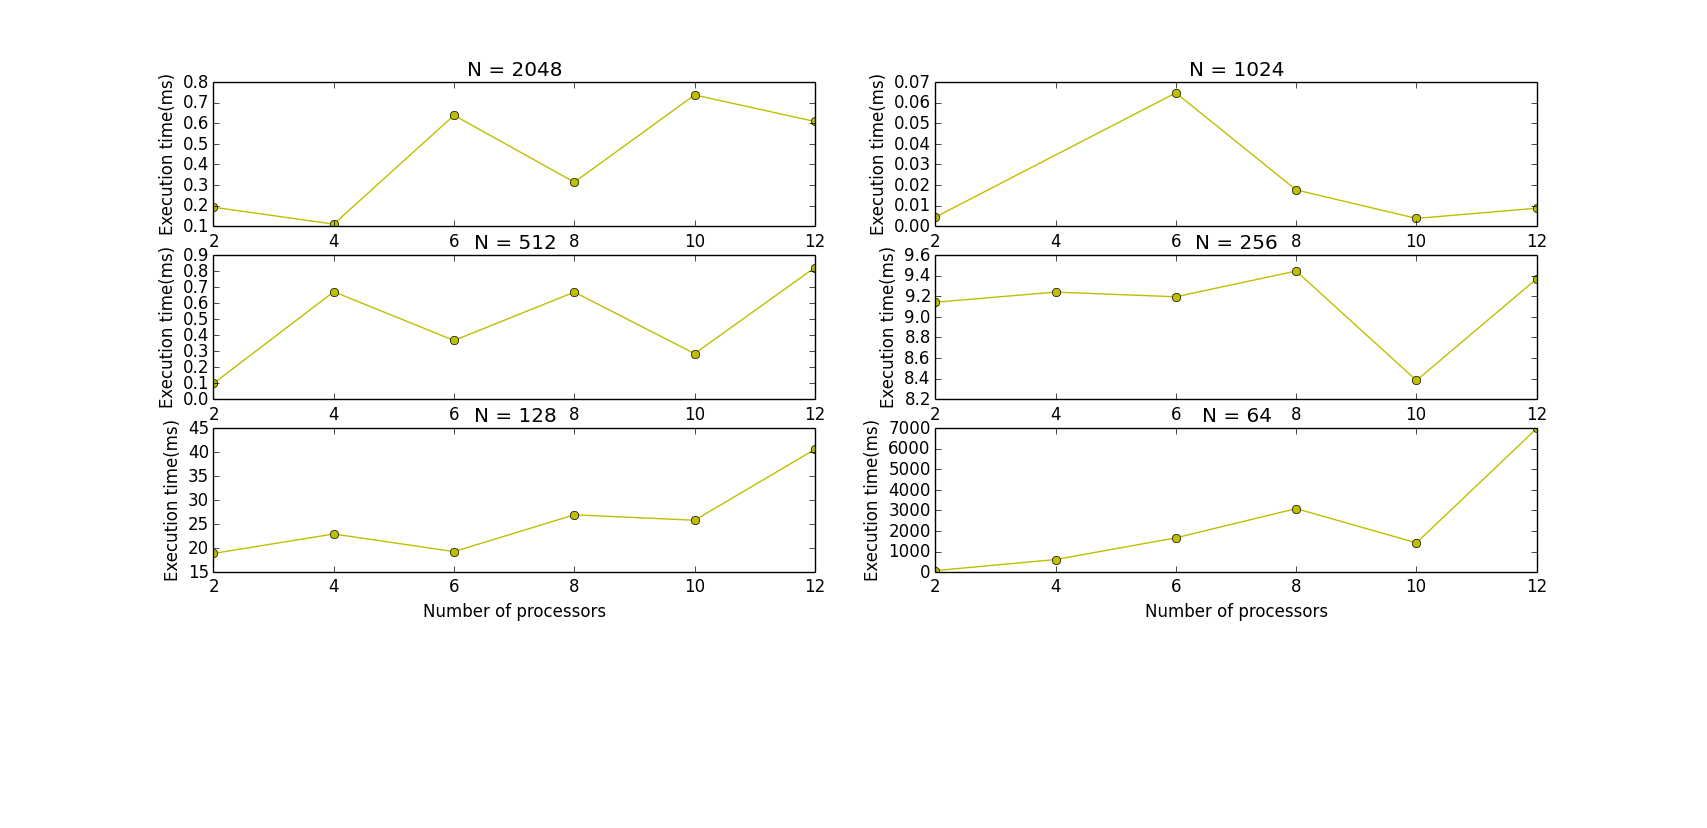
\includegraphics[scale=0.4]{../bodyo.png}
		\clearpage
		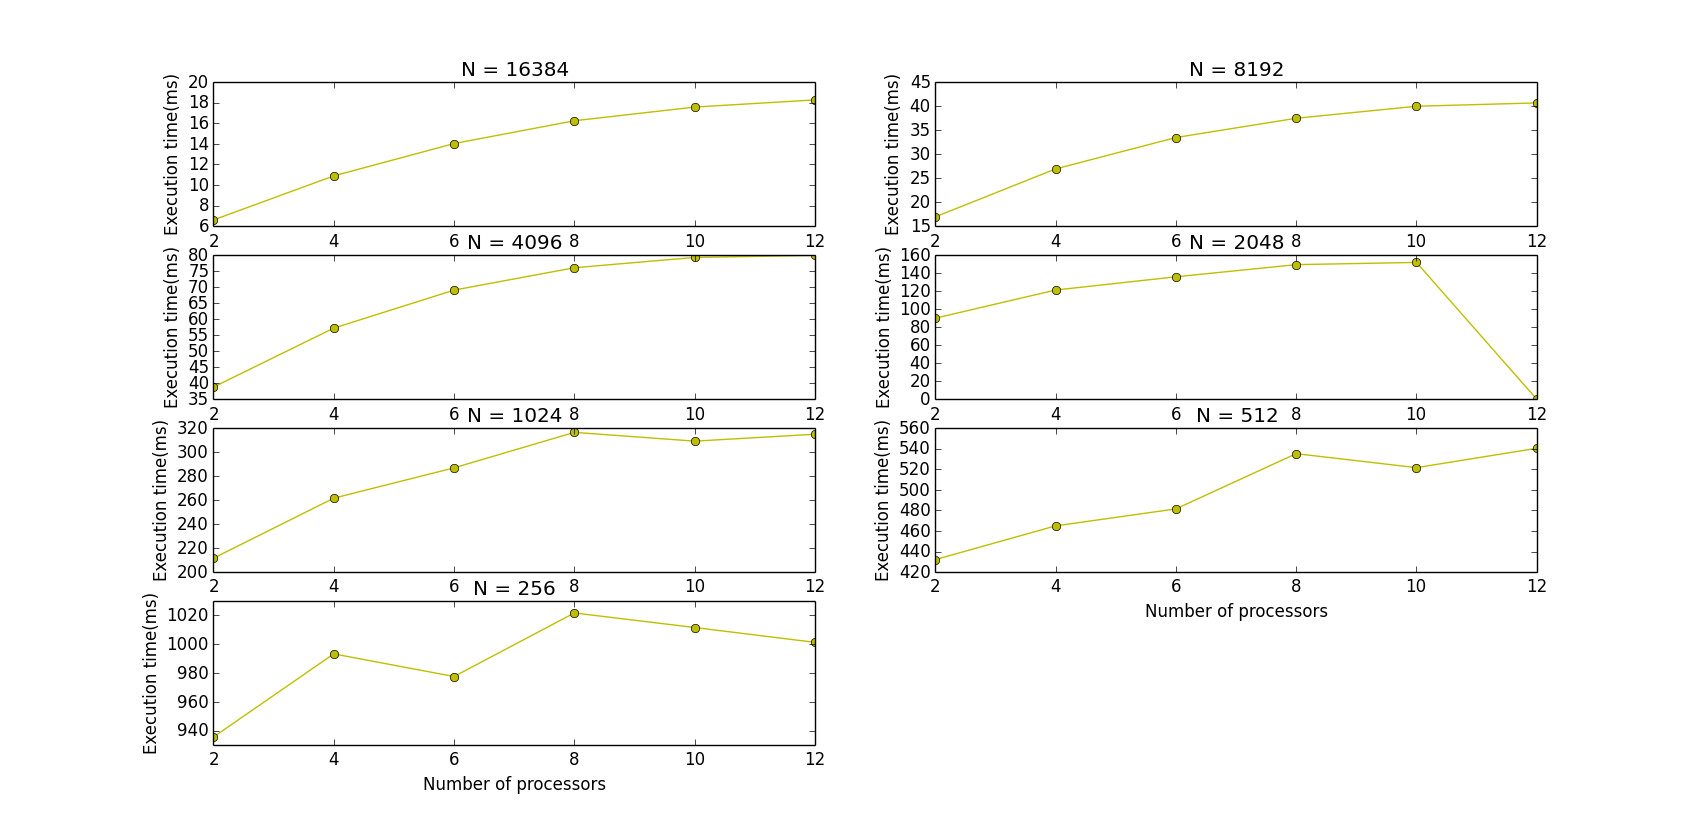
\includegraphics[scale=0.4]{../bodyp.png}
	\end{figure}
	\clearpage
	\begin{figure}[!ht]
		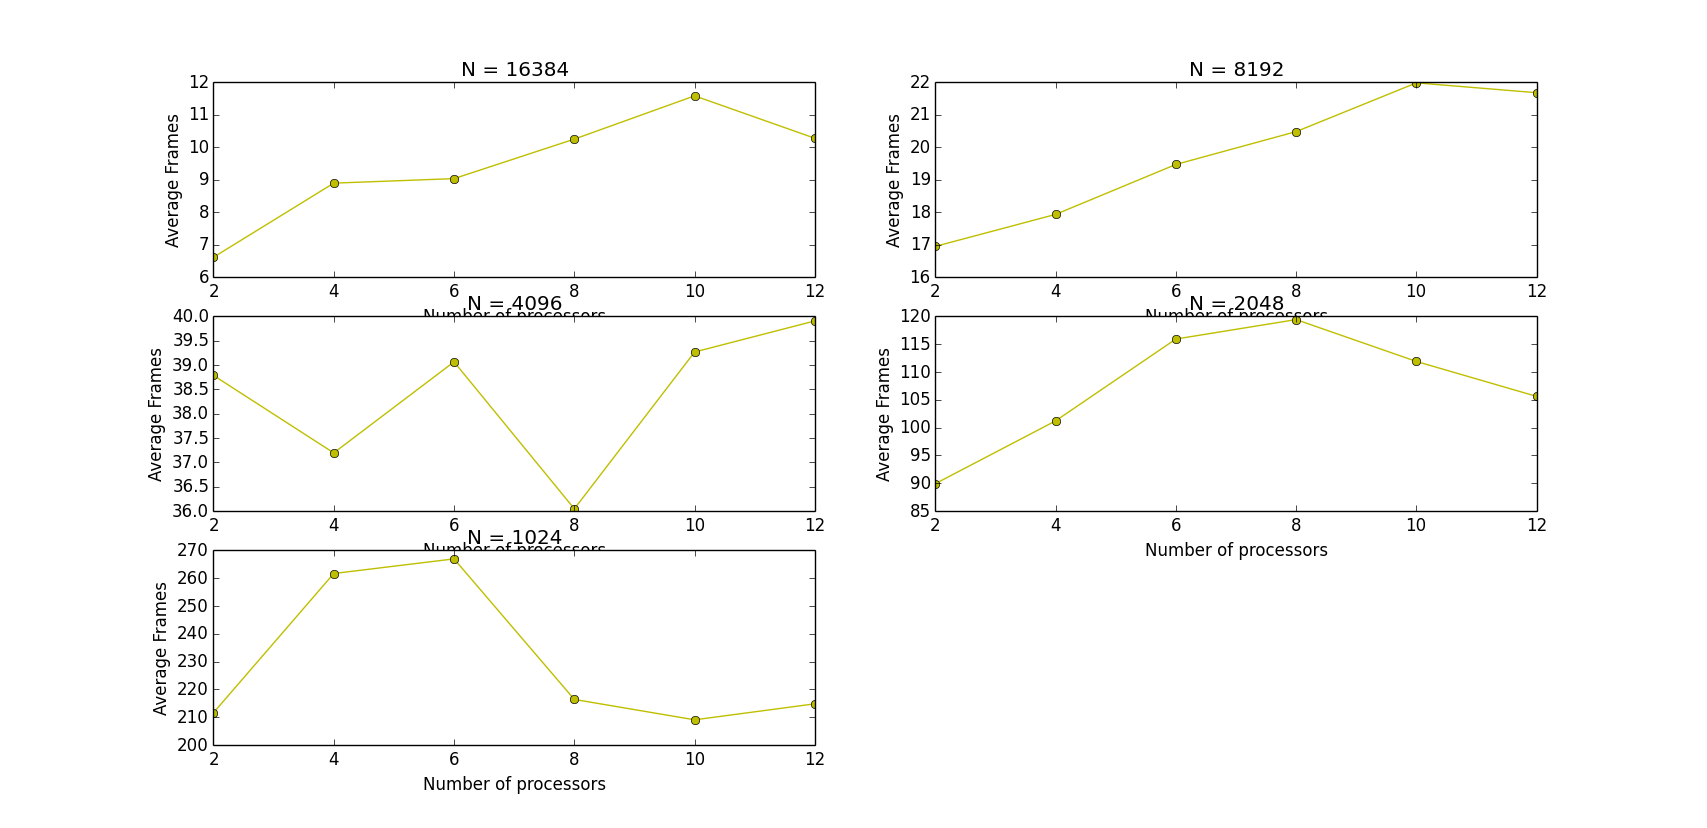
\includegraphics[scale=0.4]{../bodym.png}
	\end{figure}

\clearpage

\section{Source Code}
	\cppsrc{../../src/body.hh}
	\cppsrc{../../src/body.cc}
	\cppsrc{../../src/nbody.hh}
	\cppsrc{../../src/nbody.cc}
	\cppsrc{../../src/AABox.hh}
	\cppsrc{../../src/engine.hh}
	\cppsrc{../../src/simple.hh}
	\cppsrc{../../src/simple.cc}
	\cppsrc{../../src/bsp.hh}
	\cppsrc{../../src/bsp.cc}
	\cppsrc{../../src/worker.hh}
	\cppsrc{../../src/openmp.hh}
	\cppsrc{../../src/openmp.cc}
	\cppsrc{../../src/pthread.hh}
	\cppsrc{../../src/pthread.cc}
	\cppsrc{../../src/mpi.hh}
	\cppsrc{../../src/mpi.cc}
	\cppsrc{../../src/gtk.hh}
	\cppsrc{../../src/main.cc}
	\cppsrc{../../src/timer.hh}
	\cppsrc{../../src/timer.cc}



\clearpage
\printbibliography

\end{document}

